%%%%%%%%% wenn mehrere Anhänge vorhanden %%%%%%%%%
\begin{appendices}
    \chapter*{Anhang A}
    \addcontentsline{toc}{chapter}{A}
    \noindent \textit{Titel von Anhang A}
    
    %\begin{figure}[htb]
    %    \centering
    %        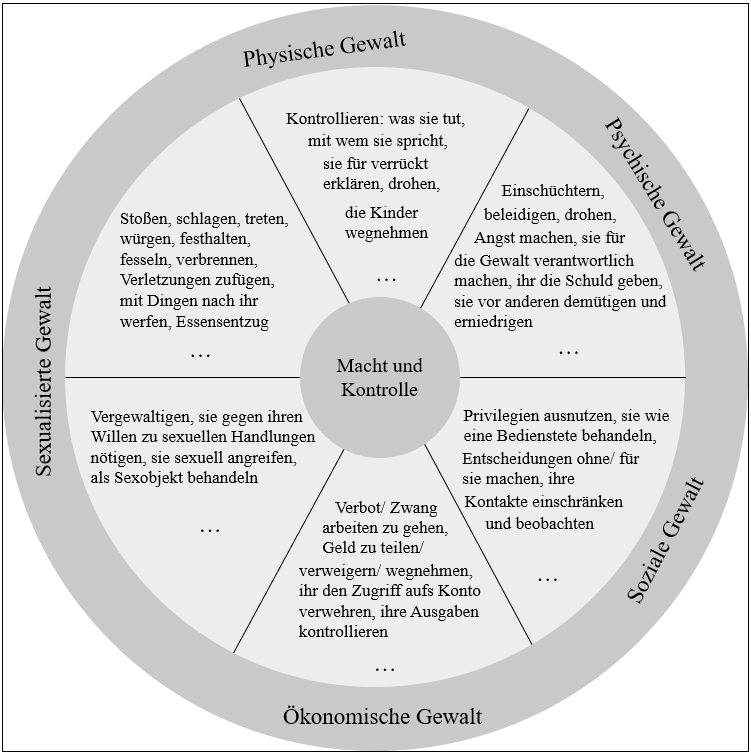
\includegraphics[width=0.8\linewidth]{Rad der Gewalt.png}
    %        \caption[Rad der Gewalt]{Rad der Gewalt \parencite{Rad_der_Gewalt}.}
    %        \label{Rad der Gewalt}
    %\end{figure}

    %%%%%%%%%%%%%%%%%%%%%%%%%%%%%%%%%%%%%%%%%%%%

    \chapter*{Anhang B}
    \addcontentsline{toc}{chapter}{B}
    \noindent \textit{Titel von Anhang B}

    Inhalt
\end{appendices}
%%%%%%%%% wenn mehrere Anhänge vorhanden %%%%%%%%%



%%%%%%%%% wenn nur 1 Anhang vorhanden %%%%%%%%%
%\chapter*{Anhang}
%\addcontentsline{toc}{chapter}{Anhang}
%\noindent \textit{Titel des Anhangs}

%Inhalt
%%%%%%%%% wenn nur 1 Anhang vorhanden %%%%%%%%%